\documentclass[11pt,a4paper]{article}
\usepackage[margin=25mm]{geometry}
\usepackage{amsmath,booktabs,tabularx,array,graphicx,microtype,xcolor}
\usepackage{tikz,pgfplots}
\usetikzlibrary{arrows.meta,positioning}
\pgfplotsset{compat=1.17}
\usepackage[hidelinks]{hyperref}
\hypersetup{pdftitle={AgriAgent Madhya Pradesh},pdfsubject={Phase III course manuscript draft}}
\setlength{\parskip}{4.5pt}
\setlength{\parindent}{0pt}
\setlength{\emergencystretch}{2em}
\raggedbottom
\newcolumntype{Y}{>{\raggedright\arraybackslash}X}
\newcolumntype{P}[1]{>{\raggedright\arraybackslash}p{#1}}
\newcommand{\code}[1]{\texttt{#1}}
\newcommand{\tp}{\mathrm{TP}}
\newcommand{\fp}{\mathrm{FP}}
\newcommand{\fn}{\mathrm{FN}}
\newif\iflocalfigures
\ifdefined\AgriLocalFigures\localfigurestrue\fi
\definecolor{agriblue}{HTML}{144B65}
\definecolor{agrigreen}{HTML}{287565}
\definecolor{agrilight}{HTML}{EBF3F5}
\tikzset{stage/.style={draw=agriblue,fill=agrilight,rounded corners=2pt,inner sep=6pt,align=center,font=\small},
         flow/.style={-{Latex[length=2mm]},draw=agriblue,thick}}

\title{\vspace{-1.3em}\textbf{AgriAgent Madhya Pradesh}\\[4pt]
\large Provenance-Aware Extraction and District-Level Agricultural Analysis}
\author{Aryan Mishra \quad Unnati Goyal \quad Yamke Sai Krishna Reddy\\
\small CS F/U 407 Artificial Intelligence, BITS Pilani\\
\small Draft author order and team identifier awaiting confirmation}
\date{24 November 2026}

\begin{document}
\maketitle
\vspace{-1em}
\begin{abstract}
Agricultural information for Madhya Pradesh is distributed across structured tables, Hindi and English documents, scanned bulletins and dynamic portals. AgriAgent makes selected observations queryable while retaining the evidence needed to trace each value to its source. A deterministic supervisor routes inputs to four specialised agents. An optional QLoRA adapter proposes fields for Agmarknet price tables, with source-cell validation before storage. The project mapped 23 inventory sources and demonstrated scoped extraction for 14. A 52-case local benchmark yielded 402 exact or tolerance-qualified field matches and macro F1 of 1.000 across four agents. The benchmark uses source fragments and does not establish performance on independent documents. On ten frozen English Agmarknet cases with 160 reference fields, the QLoRA adapter raised F1 from 0.000 to 0.677, with precision 0.955 and recall 0.525. Genuine-input unattended completion reached 11 of 17 runs and the frozen mixed multi-agent workflow cohort completed one of two runs. The 3,980-observation SQLite release passed all ten local queries, including three spatial, two temporal and two provenance queries. A 51-district balanced panel showed 58.64\% growth in observed Rabi wheat production from 2016 to 2022. The manuscript reports source coverage, licensing constraints and the instructor-dependent evaluations still outstanding.
\end{abstract}

\textbf{Keywords:} agricultural informatics, document extraction, provenance, workflow orchestration, QLoRA, SQLite, Madhya Pradesh.

\section{Introduction and problem statement}
A district crop figure becomes difficult to check when a table loses its season heading, a portal export omits a value, or a database stores a number without its source locator. This problem is concrete in Madhya Pradesh. Directorate of Economics and Statistics (DES) reports publish district production and crop-area tables, the state scheme page uses Hindi HTML, and a Sehore agrometeorology bulletin preserves measurements in a scanned image. Reading these resources requires different tools and distinct rules for establishing what a value means.

The course methodology asks teams to connect source discovery, extraction, model adaptation, database design and analyses across time and place \cite{method}. The Phase III report rubric additionally requires measured evaluation, query coverage, uncertainty and ethics \cite{phase3}. This implementation addresses a narrower engineering question: how much of a heterogeneous state corpus can be turned into auditable records using a bounded workflow, and where does adapting a language model improve extraction? The evidence combines code, input manifests, database checks, run logs, a frozen adapter comparison and a subsequent laptop verification.

\clearpage
\section{Objectives, scope and related work}
\subsection{Objectives and scope}
The system has four objectives. First, assign all Phase I sources to an extraction responsibility and record partial or pending coverage. Second, turn supported documents into typed observations with traceable locations and explicit missingness. Third, compare a fixed base model and a trained adapter on identical held-out inputs. Fourth, verify a read-only query catalogue and compare production and yield across historical districts. The core analysis covers the 2016--2022 crop-year panel and focuses on wheat, rice, soybean and maize, with chickpea present in the wider crop coverage query. Market rows, extension entries, scheme descriptions and forecast cells are separate evidence families. The project excludes personal beneficiary lookups and does not establish operational coverage of live procurement, trading, or general agricultural advice.

\subsection{Agricultural information and provenance}
DES exposes an area, production and yield reporting interface \cite{des}. Its crop and season semantics are essential when comparing reports with a bulk snapshot. The Ministry of Panchayati Raj maintains the Local Government Directory (LGD) \cite{lgd}. A contemporary district-code list supports identity validation, while the historical layer represents a different administrative vintage. The provenance design follows the practical distinction between entities and activities in W3C PROV-DM \cite{prov}: a source snapshot is an entity, processing is a run, and the numeric observation retains the source coordinates needed for verification. The implementation stores this lineage in relational tables and JSON fields.

\subsection{Extraction and tool orchestration}
Text-layer PDF parsing, table reconstruction and OCR solve different problems. The pypdf documentation explains why positioned text and image-only pages cannot be treated as ordinary character streams \cite{pypdf}. pdfplumber exposes page geometry and table extraction \cite{pdfplumber}. Tesseract provides an OCR engine \cite{tess}, while PubLayNet illustrates the availability of learned layout detection trained on a different document distribution \cite{publay}. Here, loss of text semantics and inconsistent source layouts motivate bounded tool fallbacks and language-specific OCR. A generic learned layout model was not evaluated on the Madhya Pradesh corpus.

ReAct and Toolformer provide examples of model-driven tool selection \cite{react,toolformer}. LangGraph supports explicit workflow and routing patterns \cite{langgraph}, and AgentEvals offers trajectory comparisons \cite{agentevals}. AgriAgent uses fixed routing and tool arguments for supported layouts. The optional model is limited to field proposals on one known CSV family. This design permits exact trajectory checks and reproducible failure handling at the cost of coverage when schemas drift.

\subsection{Parameter-efficient adaptation}
LoRA introduces trainable low-rank updates to frozen weights \cite{lora}. QLoRA applies this idea to a quantised base to reduce training memory \cite{qlora}. Qwen2.5 provides the base model family \cite{qwen}. The experiment tests whether supervised adaptation improves conformity to a field schema on market records. Scholarly work explains the design choices. The measured scores and scope of transfer come from the project runs.

\clearpage
\section{Agricultural sources and corpus preparation}
The inventory includes 23 entries spanning fertilizer, procurement, extension, engineering schemes, weather, statistics, insurance and markets. Every entry has an assigned responsibility or explicit exclusion. Four runtime agents cover 14 entries within declared partial scopes. Nine remain pending or excluded. Table~\ref{tab:sources} summarises actual source roles. Broader inventory labels do not identify additional implemented agents.

\begin{table}[!ht]
\small
\caption{Source families, extraction scope and audit evidence (provisional Table 1).}
\label{tab:sources}
\begin{tabularx}{\linewidth}{@{}P{.18\linewidth}P{.24\linewidth}Y@{}}
\toprule
Inventory entries & Source and supported input & Scope of retained evidence\\
\midrule
S04, S13, S14, S16 & Workflow manual, national statistical summary, crop-insurance and assistance documentation & Scoped historical operational or numerical facts. The extracted facts do not establish current scheme rates or individual eligibility.\\
S06, S08, S09 & Hindi MSP, machinery facilities and rules pages & Label--value fields, seven facility fields and three deadline facts. Five publisher blanks remain in the MSP case.\\
S10 & Image-only Sehore IMD bulletin & 15 dated forecast values checked. Forecasts are distinct from measured crop outcomes.\\
S11, S12 & DES district APY export and major-district report & 156 observations on the direct Rabi wheat report, with 104 area and production cells corroborated against the bulk panel. The ranking report supplied 52 production rows.\\
S18, S20 & e-NAM listings and licence counts & Published MP mandi entries and three count fields within the corresponding pages.\\
S21 & ICAR Krishi Vigyan Kendra directory & 162 observations from 54 historical directory entries.\\
S23 & Economic Survey PDF and derived CSV & Ten selected survey facts. The frozen release imported the derived CSV. A later bounded PDF route reproduced the ten facts directly.\\
Pending or excluded & Fertilizer, procurement, trading, service links, dashboard, telephone directory and beneficiary lookup & Template or index access alone did not establish extraction. S17 beneficiary-level lookup was excluded.\\
\bottomrule
\end{tabularx}
\end{table}

The 135-file manifest records source identifier, URL, acquisition date, language, rights status, checksum, byte size, parent and transformation. All 135 entries matched the recorded bytes during the final freeze. Acquisition code retains raw snapshots and uses provenance metadata to distinguish portal exports, mirror bytes, local rows, fragments and manually transcribed data. Dataset splits and file digests are recorded before scoring. A fresh publisher response reproduced the same missing fields in the MSP source. A CAPTCHA-protected price form and an e-NAM endpoint returning HTML could not provide eligible values. These cases remain visible in the production ledger.

The bulk crop snapshot contains 1,899 district--crop--year--season rows. Thirteen Summer production cells are absent in both the retained CSV and the direct DES follow-up. The wheat cross-check verifies a specific slice and does not establish byte identity for the full mirror. A rights review distinguishes public accessibility from permission to redistribute the exact bytes.

\clearpage
\section{System architecture and orchestration}
The entry point accepts a local file and a separate configuration covering resource limits, output directories and optional model or registry inputs. It records the source digest before extraction. The router builds the plan from file signature and supported content. The LangGraph controller executes each specialist in order, advances to a next agent when available, and retains trace entries for every attempted tool call. Figure~\ref{fig:architecture} shows the data and control paths.

\begin{figure}[!ht]
\centering
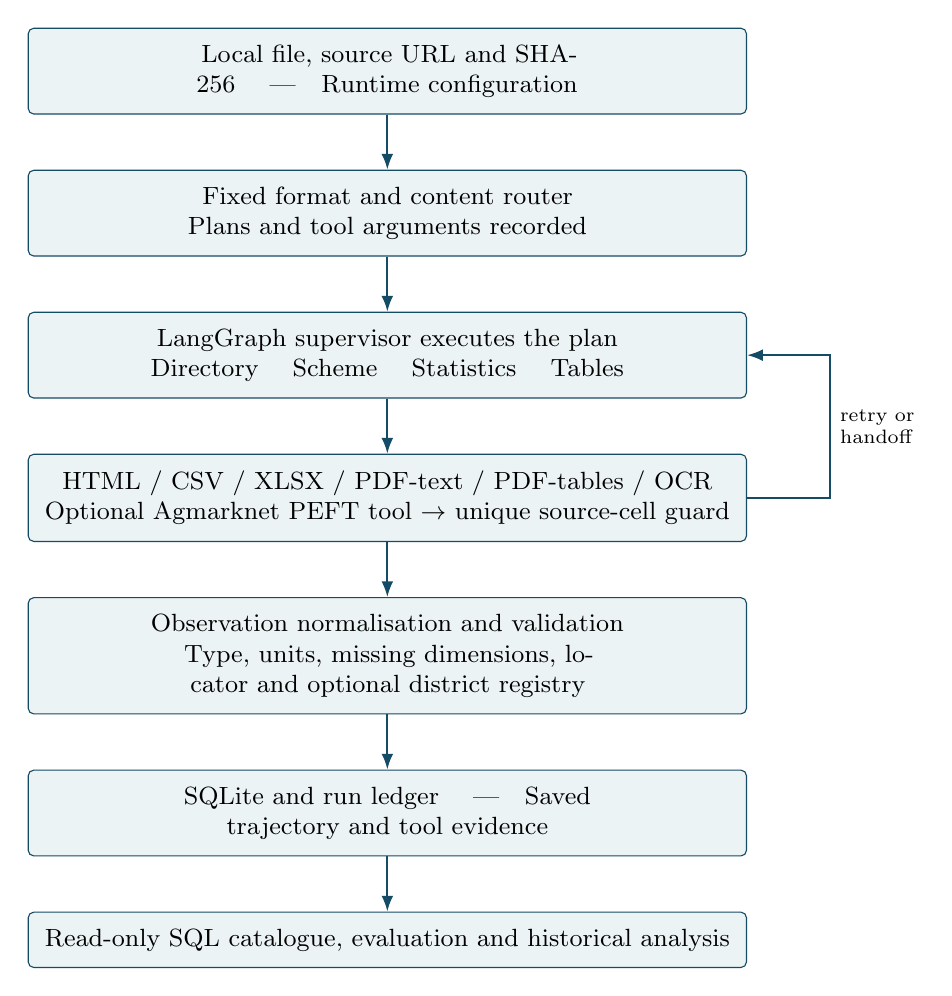
\begin{tikzpicture}[node distance=7mm]
\node[stage,text width=8.7cm] (input) {Local file, source URL and SHA-256 \quad|\quad Runtime configuration};
\node[stage,below=of input,text width=8.7cm] (router) {Fixed format and content router\\Plans and tool arguments recorded};
\node[stage,below=of router,text width=8.7cm] (agent) {LangGraph supervisor executes the plan\\Directory \quad Scheme \quad Statistics \quad Tables};
\node[stage,below=of agent,text width=8.7cm] (tools) {HTML / CSV / XLSX / PDF-text / PDF-tables / OCR\\Optional Agmarknet PEFT tool $\rightarrow$ unique source-cell guard};
\node[stage,below=of tools,text width=8.7cm] (validation) {Observation normalisation and validation\\Type, units, missing dimensions, locator and optional district registry};
\node[stage,below=of validation,text width=8.7cm] (storage) {SQLite and run ledger \quad|\quad Saved trajectory and tool evidence};
\node[stage,below=of storage,text width=8.7cm] (out) {Read-only SQL catalogue, evaluation and historical analysis};
\draw[flow] (input)--(router);
\draw[flow] (router)--(agent);
\draw[flow] (agent)--(tools);
\draw[flow] (tools)--(validation);
\draw[flow] (validation)--(storage);
\draw[flow] (storage)--(out);
\draw[flow] (tools.east) -- ++(1.05,0) |- node[pos=.25,right,font=\scriptsize,align=left] {retry or\\handoff} (agent.east);
\end{tikzpicture}
\caption{Implemented processing path. Routing, schema validation and SQLite writes are fixed decisions. Model inference occurs only on the enabled Agmarknet branch.}
\label{fig:architecture}
\end{figure}

For PDFs the usual plan is \(\langle\mathrm{Statistics},\mathrm{Tables}\rangle\). Searchable text may produce facts or yield a no-data result, at which point the table agent inspects the pages. The supervisor can terminate after a scoped policy or workflow extraction when the document-specific contract is satisfied. A transient injected tool fault returns to the same agent with at most two retries. Previously successful inspection of the same PDF can be reused within the run. Limit errors terminate processing. The pipeline records complete, partial or failed status after validation. A sequential fallback preserves the basic state transitions when LangGraph is unavailable.

A single monolithic parser would simplify dispatch but would make policy phrases, table cells and OCR failures difficult to distinguish operationally. Free-form model tool selection could accommodate unfamiliar layouts, but the declared references could no longer predict the exact tool sequence or its arguments. The explicit workflow keeps these trade-offs observable.

\clearpage
\section{Agent design and implementation}
Each agent consumes a bounded source representation and emits a common observation schema. The agent that produced a value remains distinguishable from the supervisor and from other specialists that only inspected the source.

\begin{table}[!ht]
\small
\caption{Implemented agents, tools, decisions and boundaries (provisional Table 2).}
\label{tab:agents}
\begin{tabularx}{\linewidth}{@{}P{.14\linewidth}P{.25\linewidth}Y@{}}
\toprule
Agent & Input and executed tools & Decision, output and failure boundary\\
\midrule
Directory & KVK HTML using Beautiful Soup & Find supported address, host and sanction fields, emit row-located observations, retain unresolved names and report historical directory coverage.\\
Scheme & Hindi HTML, Beautiful Soup and scoped public-source handlers & Identify policy or listing rows, preserve Hindi labels, validate numerical fields when declared, and retain blank source values as missing.\\
Statistics & Structured CSV via the Python CSV reader, or searchable PDF via pypdf & Preserve typed rows and lineage from imports. Apply bounded production, survey, policy or workflow extraction on recognised PDF patterns. Hand off unsupported document layout.\\
Tables & pdfplumber, CSV, openpyxl and Tesseract. Optional PEFT extraction & Resolve header context, detect digital/scanned pages, parse cells or group OCR word boxes. Restrict accepted predictions to unique source matches. Duplicate or unsupported candidates and missing values cannot generate new facts.\\
\bottomrule
\end{tabularx}
\end{table}

Directory rows associate historical addresses and institutional hosts with source row locators. A scheme run can be partial even when its HTML was parsed correctly. The MSP result preserved all declared fields while five source entries remained blank. The statistical CSV route inherits the survey transcription's parent and locator. The original release uses that derived input, and the separate PDF route later reproduced the scoped facts for the automation follow-up.

The tables agent inspects text and tries focused geometric extraction on selected pages. When an appropriate text layer is unavailable, it can render pages or images and reconstruct rows from OCR word boxes. Header and row context establish crop, district, period, variable and unit. This addresses both bilingual tabular records and layout-specific failures, within declared page and OCR limits. In the DES laptop run a sentence grammar returned no supported result, after which the tables agent located the 52 district production records.

For the Agmarknet model branch, deterministic parsing first establishes source candidates. A proposed tuple is accepted only when a unique source candidate satisfies the configured match. Partial model confirmation can reduce the output to confirmed rows. An unavailable model or a model producing no supported rows can fall back to the deterministic extractor. The application logs the decision and token usage when available. These semantics are important when comparing guarded application inference with the separately scored model outputs.

\clearpage
\section{Extraction, validation, provenance and database design}
\subsection{Observation representation}
A field is represented as \(o=(c,d,t,v,x,u)\), where \(c\) is crop, \(d\) district or scope, \(t\) time, \(v\) variable, \(x\) value and \(u\) unit. Provenance adds source identity, URL, SHA-256, processing run, agent, and the location of the value in the retained file. The schema supports row-and-column CSV locators, page/table/row/column PDF locators, and table or row locations for HTML. For derived inputs, the payload can carry both a local locator and an original parent locator.

Normalisation applies declared crop synonyms, district name aliases, temporal parsing and unit rules. It preserves the distinction between explicitly coded missing dimensions and source values required for a numeric observation. Compatibility is checked in the declared unit registry before field scoring. For known registry data, the pipeline can validate district codes in the relevant source scope. Unresolved district identities are left explicit. The direct ministry recheck confirmed the retained workbook, CSV and generated registry agree on 55 current codes and names. Read-only joins matched 52 of 52 historical districts, 1,886 of 1,886 panel rows and 52 of 52 historical geometry names. The result does not reconstruct administrative changes.

\subsection{Relational representation}
The SQLite implementation uses foreign keys \cite{sqlite}, explicit validation status and a uniqueness constraint. Each source identifies a hash-pinned snapshot. A run identifies a processing attempt and links to a source. An observation relates to both and retains original payload fields. An attempts row records duplicate and insertion counts per run. The natural key is
\[
(\mathrm{source},\mathrm{locator},c,d,t,v).
\]
This makes replay of the same source location idempotent at the observation level. Values extracted independently from distinct source files can coexist because their lineage differs.

\begin{figure}[!ht]
\centering
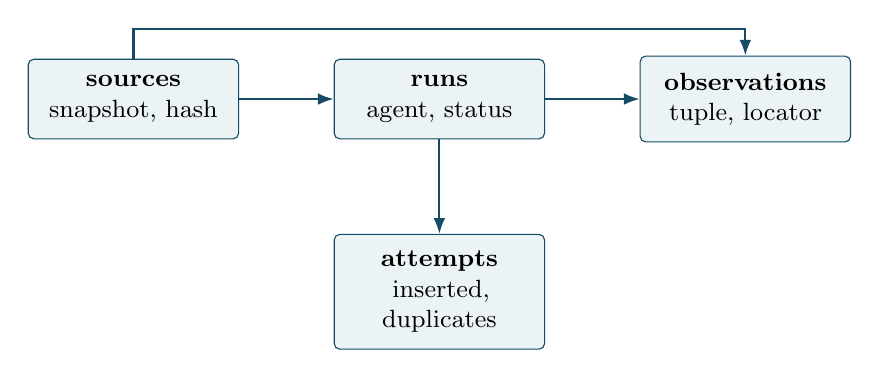
\begin{tikzpicture}[node distance=12mm]
\node[stage,text width=2.25cm] (s) {\textbf{sources}\\snapshot, hash};
\node[stage,text width=2.25cm,right=of s] (r) {\textbf{runs}\\agent, status};
\node[stage,text width=2.25cm,right=of r] (o) {\textbf{observations}\\tuple, locator};
\node[stage,text width=2.25cm,below=of r] (a) {\textbf{attempts}\\inserted, duplicates};
\draw[flow] (s)--(r);
\draw[flow] (r)--(o);
\draw[flow] (r)--(a);
\draw[flow] (s.north) -- ++(0,.38) -| (o.north);
\end{tikzpicture}
\caption{Logical SQLite relationships. Arrows run from parent records to their dependent records.}
\label{fig:schema}
\end{figure}

The release contains 3,980 observations, including directory, scheme, survey and crop statistics. The analytical view selects the pinned district crop CSV, filters valid area and production, and groups by source, district, crop, crop year and season. It requires exactly one area and one production row for an eligible pair. The resulting 1,886 pairs support historical district analysis. A database-wide duplicate count of zero differs from an insertion-attempt count, as a rerun can encounter existing natural keys and correctly insert nothing.


\clearpage
\section{QLoRA fine-tuning and frozen comparison}
\subsection{Training and separation}
The base was \code{Qwen2.5-1.5B-Instruct}. Its pinned revision was
\begin{center}
\small\texttt{989aa7980e4cf806f80c7fef2b1adb7bc71aa306}.
\end{center}
Training comprised 72 examples and 1,152 target field tuples derived from English Agmarknet records with 2008--2010 parent years. Prompts supplied the source content and requested a schema-conforming sequence. Completions used normalised variables and units for arrivals and price. The ten held-out cases in the frozen M18 lock contained 160 reference tuples, with source parents from 2011, 2013 and 2017. The package excluded the held-out answer files. Exact input and parent-file hashes did not overlap between the training and held-out sets. This check does not establish whether base-model pretraining contained related public material.

For a targeted linear transformation, the implementation keeps the base operation frozen and trains a scaled low-rank update:
\begin{equation}
W_{\mathrm{eff}}=\operatorname{dequant}_{\mathrm{NF4}}(W_q)+\frac{\alpha}{r}BA,
\quad
B\in\mathbf{R}^{d_\mathrm{out}\times r},\
A\in\mathbf{R}^{r\times d_\mathrm{in}}.
\end{equation}
With rank \(r=16\) and \(\alpha=32\), the trained matrices correct the representation without updating the full checkpoint. The adapter targets query, key, value and output projections and applies dropout 0.05. The supervised objective is causal next-token negative log-likelihood over the rendered training sequence with padding excluded. The exported configuration records \code{assistant\_only\_loss=false}, so the experiment is not reported as applying assistant-only masking.

\begin{table}[!ht]
\small
\caption{Retained training and decoding configuration.}
\begin{tabularx}{\linewidth}{@{}P{.32\linewidth}Y@{}}
\toprule
Setting & Actual run\\ \midrule
Compute and precision & Tesla T4; base compressed to 4-bit NF4 and FP16 computation in the quantised layers\\
Adaptation & Rank 16, scale parameter 32, dropout 0.05; \code{q\_proj}, \code{k\_proj}, \code{v\_proj}, \code{o\_proj}\\
Optimisation & Fused AdamW, learning rate \(2\times10^{-4}\), linear schedule, no warm-up ratio, gradient checkpointing enabled\\
Batch and length & Device batch one, accumulation eight, three epochs, seed 7, maximum sequence 4,096; longest training sequence 1,381 tokens\\
Frozen evaluation & Greedy decoding, up to 1,280 generated tokens, identical locked cases and reference set for both conditions\\
\bottomrule
\end{tabularx}
\end{table}

The runner saved the quantised base predictions before training. After training, it reloaded the adapter against a fresh instance of the same pinned quantised checkpoint and used the same tokenizer, prompts and decoding settings. The run completed 27 optimiser steps in 267.11 trainer seconds. First and final logged losses were 0.7282 and 0.2829, with mean training loss 0.4415. These are training diagnostics. The adapter has 4,358,144 parameters across 224 finite tensors, with all 112 LoRA B tensors nonzero. The archive check matched 18 extracted files and verified all 17 manifest-designated hashes. M18 uses the original frozen predictions. Application integration is evaluated separately because it adds a unique-source guard and uses a local CPU configuration.

\clearpage
\section{Phase II evaluation methodology}
The official protocol distinguishes source coverage, field-level extraction, trajectory, workflow, automation and database outcomes \cite{phase2}. The local extraction benchmark has 52 cases across four agents. Directory and scheme cases are source fragments. The ten statistics cases exercise scoped survey values through the structured CSV importer. The tables cases exercise deterministic parsing of source-derived Agmarknet inputs. The independently reviewed surprise inputs and values required for assessed M5 were unavailable.

\subsection{Field matching and aggregation}
A predicted field and a reference field are eligible to match when their normalised crop, location, time and variable agree. Integer values and codes require exact equality under the declared rules. For decimal quantities after compatible unit conversion, test
\[
|x_{\mathrm{pred}}-x_{\mathrm{ref}}|\leq 0.01\,|x_{\mathrm{ref}}|.
\]
A zero reference therefore requires equality. The scorer consumes a reference at most once in prediction order. With unmatched predictions counted as \(\fp\) and unmatched references as \(\fn\), the report uses
\[
P=\frac{\tp}{\tp+\fp},\qquad
R=\frac{\tp}{\tp+\fn},\qquad
F_1=\frac{2\tp}{2\tp+\fp+\fn}.
\]
Extraction and agent scores pool counts within each of the four agents first, then compute the equal-weight mean \(\bar m=\frac14\sum_{a=1}^{4}m_a\). Pooled source-group and language results describe their own denominators. The same tuple method scores both model conditions on the paired, frozen tables-only cohort.

\begin{table}[!ht]
\small
\caption{Local extraction benchmark subgroups. Subgroup rows overlap other groupings.}
\label{tab:subgroups}
\begin{tabularx}{\linewidth}{@{}Yrrcc@{}}
\toprule
Grouping & Cases & TP & FP/FN & F1\\ \midrule
Directory & 10 & 30 & \(0/0\) & 1.000\\
Scheme & 10 & 10 & \(0/0\) & 1.000\\
Statistics & 10 & 10 & \(0/0\) & 1.000\\
Tables & 22 & 352 & \(0/0\) & 1.000\\
Document / Database & \(20/32\) & \(40/362\) & \(0/0\) each & 1.000 each\\
English / Hindi & \(42/10\) & \(392/10\) & \(0/0\) each & 1.000 each\\
Overall pooled & 52 & 402 & \(0/0\) & 1.000\\
Equal-agent macro & 4 agents & -- & -- & 1.000\\
\bottomrule
\end{tabularx}
\end{table}

Tool and argument checks compare the observed sequence against declared calls, and AgentEvals performs strict trajectory matching with exact arguments. Groundedness resolves the local source cells and checks the normalised field tuple. These are deterministic checks. They avoid the use of an uncalibrated language-model judge and depend on the accuracy and coverage of the reference files. The Hindi subset consists of scheme examples. It should be read alongside the separate OCR experiments rather than as an estimate of Hindi OCR accuracy.

\clearpage
\section{Phase II results for M1--M18}
Table~\ref{tab:metrics} uses the current evaluation snapshot. Floors and targets appear for context. No course points, gate decisions or instructor-confirmed values are inferred.

\begin{table}[!ht]
\small
\setlength{\tabcolsep}{4pt}
\renewcommand{\arraystretch}{1.08}
\caption{Phase II measured and pending results. Bounds are protocol floor to target.}
\label{tab:metrics}
\begin{tabularx}{\linewidth}{@{}P{.28\linewidth}P{.17\linewidth}Y@{}}
\toprule
Metric & Bounds & Result and denominator\\ \midrule
M1 Source mapping & .50 to 1.00 & \(23/23=1.000\) mapped.\\
M2 Implementation & .20 to .60 & \(14/23=0.609\), within documented scopes.\\
M3 Field F1 & .50 to .85 & 1.000 macro across four agents, 402 TP over 52 local cases.\\
M4 Provenance & .60 to .95 & \(402/402\) locators resolved locally, 1.000 macro. Evaluator sampling pending.\\
M5 Surprise F1 & .30 to .75 & Pending three instructor items and checked keys.\\
M6 Tool selection & .60 to .90 & \(52/52\) matching calls, 1.000 macro.\\
M7 Tool arguments & .60 to .90 & \(52/52\) matching calls, 1.000 macro.\\
M8 Trajectory match & .50 to .80 & \(52/52\) strict reference matches, 1.000 macro.\\
M9 Task completion & .50 to .90 & \(52/52\) complete and schema-valid, 1.000 macro.\\
M10 Groundedness & .70 to .95 & \(402/402\) supported field tuples, 1.000 macro.\\
M11 Workflow success & .50 to .90 & \(1/2=0.500\) planned mixed local workflows complete. Separate fault evidence in Sec.~\ref{sec:repro}.\\
M12 Automation & .30 to .80 & Genuine inputs \(10/17=0.588\), paired rerun \(11/17=0.647\).\\
M13 Redundant calls & .50 to .10 & \(0/52\) redundant calls and zero retries in controlled benchmark.\\
M14 Mandatory fields & .80 to 1.00 & \(3980/3980=1.000\), including explicit missing codes.\\
M15 Validation pass & .70 to .98 & \(3975/3980=0.9987\) under frozen release rules.\\
M16 Duplicate rows & .10 to .00 & \(0/3980\) share the declared observation key.\\
M17 Live trace-back & 1 to 3 & Pending three evaluator-selected rows and source checks.\\
M18 Adapter comparison & Same held-out cases & \(+0.677419\) F1 over ten cases, 160 reference fields, zero exact input and parent overlap.\\
\bottomrule
\end{tabularx}
\end{table}

The frozen M11 cohort includes the partial Economic Survey PDF and one complete synthetic district APY PDF. The fault-injected variants are reported separately. The cohort is too small to estimate general workflow reliability.

M12 divides complete runs requiring no intervention by all attempts, including partial, failed and manually assisted cases. The paired rerun preserved all 17 slots and directly processed the same survey facts from the original PDF. It retained four partial and two failed cases. Meeting the 80\% target with this denominator requires 14 unattended completions. The separate positive benchmark completed 52 of 52 on its controlled inputs. For M13 the protocol numerator is actual tool and model calls minus the reference count. Production references are incomplete, so the benchmark count cannot be generalised. The M14--M16 measurements describe the frozen release, which predates direct ministry registry verification.

\clearpage
\section{Error analysis and adapter performance}
\begin{table}[!ht]
\small
\caption{Frozen M18 comparison on the same ten English Agmarknet inputs.}
\label{tab:adapter}
\begin{tabularx}{\linewidth}{@{}Yrrrrrr@{}}
\toprule
Condition & TP & FP & FN & Precision & Recall & F1\\ \midrule
Pinned base & 0 & 56 & 160 & 0.0000 & 0.0000 & 0.0000\\
QLoRA adapter & 84 & 4 & 76 & 0.9545 & 0.5250 & 0.6774\\
\bottomrule
\end{tabularx}
\end{table}

The base produced literal source headers or source-form dates that did not match the declared tuples. It also had one JSON decode failure. The adapter decoded all ten cases and fully matched four. Five other cases retained four correct fields each. One case used state-level location where district-level values were expected and accounts for all four false positives. The gain therefore reflects improved schema conformity and recovery of reference fields under the fixed scorer. A low base score in this comparison provides no evidence about unscored semantic answers. The adapter still missed 76 reference fields.

On the laptop, the exact base and adapter hashes were verified before use. The application trace recorded a successful \code{llm.peft\_extraction} call, 347 input and 292 generated tokens, and a duration of 276.78 seconds. Its unique-source guard confirmed 4 of 16 fields, with zero unmatched predicted fields. The run was partial (\(P=1.00\), \(R=0.25\) on that case). The deterministic control returned all 16 fields. Differences between the guarded unquantised CPU path and the exported Colab predictions prevent attribution of the discrepancy to any single component.

\begin{table}[!ht]
\small
\caption{Measured extraction-tool checks on retained project inputs.}
\begin{tabularx}{\linewidth}{@{}P{.31\linewidth}Y@{}}
\toprule
Check & Observation and unit\\ \midrule
PDF text extraction & The 20-page Economic Survey had text on 17 pages for both pypdf (22,368 characters, 0.969 s) and pdfplumber (21,834 characters, 3.806 s).\\
Hindi legacy text layer & On a 35-page manual, neither native tool recovered both specified footer words. Tesseract \code{hin} recovered both on 26/35 pages at 300 dpi.\\
Hindi image-region OCR & Three regions yielded character error 3.45\%, word error 13.04\%, and one exact region match. Native text matched none.\\
English image-only bulletin & 15/15 dated values matched in the revised Sehore run. The retained lower-resolution pilot misread one temperature.\\
\bottomrule
\end{tabularx}
\end{table}

Text volume measures readable output volume and does not establish field accuracy. OCR error rates use edit distance divided by the corresponding reference character or word count. The four tool checks use different units and samples. Together they show why deterministic text, geometric extraction and OCR are complementary. The small samples do not support an estimate for arbitrary Hindi documents or unobserved English layouts.

Production failures had different causes. The Hindi MSP row set contained five publisher blanks, and the bulk production file and Summer rice and maize exports lacked production cells. The mandi rates form required a CAPTCHA, and the e-NAM endpoint did not return usable state rows. In all six remaining unsuccessful cases, attempting inference over the absent content would compromise provenance.

\clearpage
\section{Phase III read-only query system}
The Phase III methodology calls for ten live queries, including spatial, temporal and source-location questions \cite{method,phase3}. The implementation exposes ten fixed SQL queries on a read-only SQLite connection. Analysts choose a catalogue identifier. SQL supplies explicit crop, season and year conditions, stable ordering, eligibility rules and provenance joins. The model does not generate SQL. Spatial questions are district comparisons or rankings, with geometry used separately for analysis.

\begin{table}[!ht]
\small
\setlength{\tabcolsep}{4pt}
\caption{Ten locally verified queries, with result sizes and diagnostic examples.}
\label{tab:queries}
\begin{tabularx}{\linewidth}{@{}llrY@{}}
\toprule
ID & Category & Rows & Question and observed example\\ \midrule
q01 & Spatial & 5 & Largest 2022 Rabi wheat producers. Dhar leads at 1,773,206 t.\\
q02 & Spatial & 5 & Highest observed 2022 Kharif soybean yields. Top displayed yield is 1.605 t/ha in Dhar.\\
q03 & Temporal & 7 & Annual Rabi wheat production and district count. 2016 contains 51 districts and 21.916 million t.\\
q04 & Temporal & 7 & Sehore Rabi wheat yield by year. The 2016 value is 3.388 t/ha.\\
q05 & Provenance & 1 & Sehore 2022 wheat production, 1,177,873 t. Parent mirror CSV line 397682, column Production, with local locator and hash.\\
q06 & Comparison & 3 & Area-weighted 2022 Kharif yields and crop coverage. Maize yields 3.191 t/ha with 48 districts.\\
q07 & Spatial & 5 & Largest matched district changes in Rabi wheat output, 2016 to 2022. Dhar increases by 1,022,206 t.\\
q08 & Comparison & 1 & In 48/48 eligible paired districts, 2022 Kharif maize yield exceeds soybean yield.\\
q09 & Coverage & 35 & District counts with available area and production. The 2016 chickpea count is 51.\\
q10 & Provenance & 4 & Four wheat and rice estimates with original source. The Economic Survey observations point to physical PDF page 7.\\
\bottomrule
\end{tabularx}
\end{table}

Verification compares complete ordered results against retained expected rows. The expected-query script recomputes the panel cases from the source data, while the survey check follows the retained transcription and its PDF locators. All ten matched on the existing, rebuilt and restored release. The catalogue covers three spatial, two temporal, two provenance, two comparison and one coverage question. The workbook, backup and query checks support a technically reproducible demonstration. The evaluator's live verification remains pending.

The q05 and q10 paths illustrate different provenance mechanisms. The first joins a production observation to the source snapshot and carries the original CSV cell reference. The second preserves the distinction between the ingested transcription and the source PDF page. Source pointers aid review even when redistribution of a retained file is limited.


\clearpage
\section{Temporal agricultural analysis}
For a district \(d\), crop \(c\), crop year \(t\) and season \(s\), let \(P_{dcts}\) be production in tonnes and \(A_{dcts}\) harvested area in hectares for a valid observed pair. District yield and area-weighted aggregate yield in an eligible district set \(D\) are
\begin{align}
Y_{dcts}&=P_{dcts}/A_{dcts}, \qquad A_{dcts}>0,\\
\bar Y_{cts}(D)&=\frac{\sum_{d\in D}P_{dcts}}{\sum_{d\in D}A_{dcts}}.
\end{align}
The aggregate is the mean of district yields weighted by area. Eligibility requires valid production and positive observed area. The 13 Summer blanks do not become zero production. For wheat trends, \(D\) is the intersection of districts with eligible Rabi wheat observations in every crop year from 2016 to 2022.

\begin{figure}[!ht]
\centering
\iflocalfigures
  \includegraphics[width=.87\linewidth,height=5.6cm,keepaspectratio]{../../output/analysis/wheat_yield_series.png}
\else
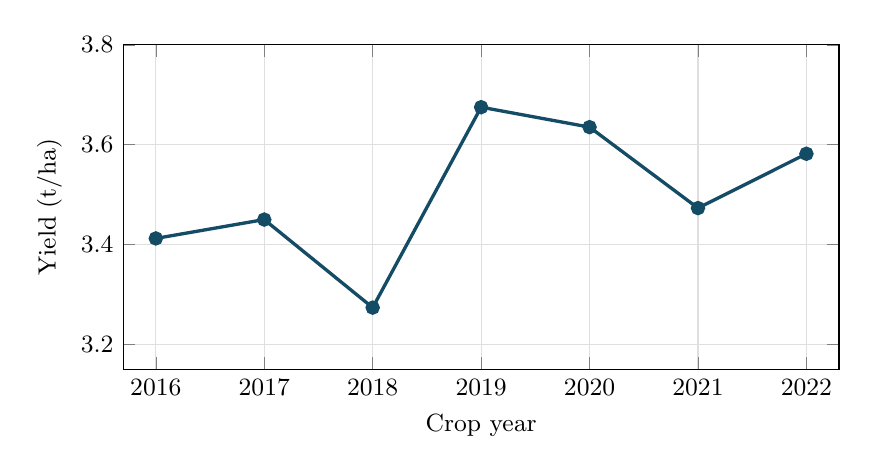
\begin{tikzpicture}
\begin{axis}[width=.88\linewidth,height=5.7cm,xlabel={Crop year},ylabel={Yield (t/ha)},
xmin=2015.7,xmax=2022.3,ymin=3.15,ymax=3.8,xtick={2016,2017,2018,2019,2020,2021,2022},
xticklabel style={/pgf/number format/1000 sep={}},grid=major,grid style={gray!25},
tick label style={font=\small},label style={font=\small}]
\addplot[agriblue,very thick,mark=*] coordinates {
(2016,3.4121) (2017,3.4499) (2018,3.2734) (2019,3.6752)
(2020,3.6352) (2021,3.4729) (2022,3.5818)};
\end{axis}
\end{tikzpicture}
\fi
\caption{Area-weighted Rabi wheat yield on the same 51 districts over seven years. The standard draft redraws the aggregate series. The local figure build uses the repository chart.}
\label{fig:wheat}
\end{figure}

\subsection{Rabi wheat output and yield over time}
Observed Rabi wheat production on the 51-district panel increased from 21,916,000 t in 2016 to 34,767,911 t in 2022, a gain of 58.64\%. Forty-six districts recorded increases. Dhar had the largest gain at 1,022,206 t. Weighted yield rose from 3.412 to 3.582 t/ha, about 4.97\%. The yield series was uneven and peaked in 2019 at 3.675 t/ha (Fig.~\ref{fig:wheat}).

The production increase is much larger than the increase in aggregate yield. The identity \(\sum P=\bar Y\sum A\) gives a reported area increase from 6.423 million ha to 9.707 million ha (51.13\%). This decomposition cannot distinguish physical expansion from reporting changes or identify the causes of either change. The balanced 2022 total differs from the all-eligible district total returned by q03 because q03 uses each year's available district set.

\clearpage
\section{Spatial analysis and paired crop relationships}
The historical geometry uses 52 Survey of India district features published through a service attributed to Survey of India \cite{boundary}. The pipeline joins canonical district names and keeps the present-day LGD check separate. Niwari has a geometry but no eligible mapped wheat observation in 2016--2018, leaving 51 of 52 coloured districts in each of those years. Coverage is 52 of 52 from 2019 to 2022. Maihar, Mauganj and Pandhurna occur in the 55-district register outside the historical layer. The comparison uses one fixed geometry layer throughout. Uncoloured districts indicate unavailable data rather than a numeric zero.

\begin{figure}[!ht]
\centering
\iflocalfigures
  \includegraphics[width=.47\linewidth,height=6.1cm,keepaspectratio]{../../output/analysis/wheat_yield_map_2016.png}
  \hfill
  \includegraphics[width=.47\linewidth,height=6.1cm,keepaspectratio]{../../output/analysis/wheat_yield_map_2022.png}
\else
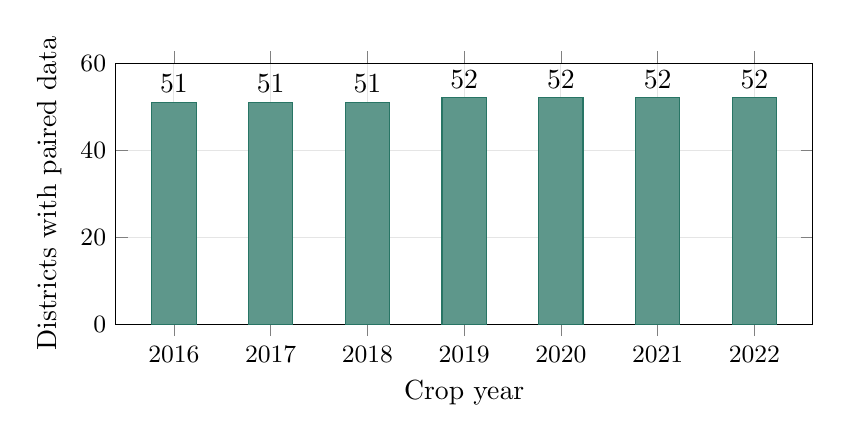
\begin{tikzpicture}
\begin{axis}[width=.86\linewidth,height=4.9cm,ybar,bar width=16pt,
xlabel={Crop year},ylabel={Districts with paired data},ymin=0,ymax=60,
symbolic x coords={2016,2017,2018,2019,2020,2021,2022},xtick=data,
nodes near coords,grid=major,grid style={gray!20},tick label style={font=\small}]
\addplot[fill=agrigreen!75,draw=agrigreen] coordinates {
(2016,51) (2017,51) (2018,51) (2019,52) (2020,52) (2021,52) (2022,52)};
\end{axis}
\end{tikzpicture}
\fi
\caption{Observed wheat map coverage on the historical 52-feature layer. The local review build shows the first and last retained maps. The default figure summarises coverage without embedding the boundary shapes.}
\label{fig:maps}
\end{figure}

\subsection{Paired district yields}
For crop pairs, each \(i\) is a district with eligible observations of both crops in the specified season and year. Pearson correlation uses
\[
r=\frac{\sum_{i=1}^{n}(x_i-\bar x)(y_i-\bar y)}
{\sqrt{\sum_{i=1}^{n}(x_i-\bar x)^2\sum_{i=1}^{n}(y_i-\bar y)^2}}.
\]
In 2022 Kharif, the paired maize and soybean yields gave \(r=0.2244\) across 48 districts. Maize yield exceeded soybean yield in all 48 pairs. A difference in the level of crop yield can coexist with a weak correlation in the geographic ranking. For 2022 Rabi wheat and Kharif rice, \(r=0.1652\) across 52 districts. This second association compares two seasons in a common crop year. Neither association controls for soil, water access or management.

\iflocalfigures
\begin{figure}[!ht]
\centering
\includegraphics[width=.68\linewidth,height=4.0cm,keepaspectratio]{../../output/analysis/maize_soybean_yield.png}
\caption{Retained local scatterplot of paired 2022 Kharif maize and soybean yields (\(n=48\)).}
\end{figure}
\else
The existing local scatterplot documents all 48 paired observations. The retained animation contains seven annual wheat-map frames. Approved display of the original maps and animation depends on the terms governing the exact historical layer.
\fi

\clearpage
\section{Reproducibility, automation and fault recovery}
\label{sec:repro}
\subsection{Reproduction and integrity}
The Windows verification used a fresh Python 3.12 environment, the declared requirements, and Tesseract English and Hindi language packs. Dependency checking succeeded. In a second local working copy with no previous outputs, the main extraction, build and query entry points ran. The isolated release builder produced 3,980 observations. The SQL dump restored to the same count with SQLite integrity and foreign-key checks passing. The final regression suite passed 62 of 62 tests. These checks provide evidence on one platform and do not replace the course's clean-machine procedure.

\begin{table}[!ht]
\small
\caption{Artifact and verification boundary for the principal experiments.}
\begin{tabularx}{\linewidth}{@{}P{.25\linewidth}Y@{}}
\toprule
Artifact & Verification boundary\\ \midrule
Corpus and release & 135 manifest entries and all 33 selected protected-file digests matched. Hold rights-restricted snapshots and derived tables in approved storage.\\
Phase II measures & Case rows, computed scopes and separate genuine-input ledgers retain their original denominators. Later owner runs do not alter the frozen cohorts.\\
QLoRA and laptop & Pinned checkpoint and adapter digests, training configuration, holdout lock, exported predictions and a separate guarded laptop trace are retained.\\
Phase III queries & Ten complete ordered results checked on retained, rebuilt and restored copies. The investigator can inspect source-linked q05 and q10 outputs.\\
\bottomrule
\end{tabularx}
\end{table}

\subsection{Fault recovery and observed latency}
The verified laptop baseline used a real DES production report. It yielded 52 records in 4.66 seconds and stored 52 observations. Five sampled values matched the original page 1 table cells. The injected run recorded the statistics-to-tables hand-off, one failure of \code{pdfplumber.extract\_tables}, one successful retry, 52 records and zero final errors in 7.73 seconds. A repeat against the same database encountered all 52 natural keys and inserted no duplicates. These are single-run times under the observed laptop conditions, without an estimate of timing variance.

The owner reports visualising the supervisor, hand-off and retry in LangSmith. The local trajectory was retained and verified. A remote trace link or export was not available for independent inspection. The fault test is separate from the frozen M11 mixed-cohort denominator. The surprise-run harness can record artifacts before an answer key is supplied. It preserves file hashes, stores status and later scores the saved extracts.

Automation improves when the same source facts can be extracted directly from an eligible report. Remaining bottlenecks include access controls, unavailable responses and publisher blanks. They require supported feeds, clarification of data semantics, or a genuine corrected publication.

\clearpage
\section{Limitations, ethics and future work}
\subsection{Measurement and implementation limits}
The local 1.000 macro F1 measures repeatability on source fragments and simple trajectories. Shared parents and development visibility limit external validity. Independent reference and trajectory review remains pending. The M18 input and parent digests establish separation from this experiment's training set. Base pretraining exposure remains unknown. The 76 missed fields and the separate partial laptop run justify independent assessment of guarded model inference.

Implementation limits include brittle layout rules, narrow OCR checks, constrained access to dynamic portals and incomplete unattended processing. The two-case workflow cohort cannot characterise reliability. A broader frozen cohort should assess repeated runs, layout shift, latency and errors.

\subsection{Analytical validity and licensing}
The panel is historical and uses a fixed boundary layer, exact crop and season eligibility, and name-level district joins. Changing boundaries, crop mix, weather, irrigation and missingness can affect the measured relationships. Paired correlations and changes in totals are descriptive. They do not support causal interpretation, prediction or farm-specific recommendations.

The manifest distinguishes source lineage from licensing. Government open data terms apply to qualifying datasets published under those terms \cite{godl}. Exact permissions for the historical crop mirror, direct portal exports, Agmarknet derivatives and boundary layer remain subject to review. The default manuscript contains original diagrams and plots of reported aggregates. Source snapshots, raw model outputs, registry bytes, original figures with unresolved rights, and trained weights stay in their controlled locations. The project excludes beneficiary-level records and avoids publishing credentials, local absolute paths and unreviewed traces. Attribution and course IP requirements must be checked before artifact release.

\subsection{Next evaluations and team confirmation}
Pending are three unseen instructor items including Hindi, three selected trace-backs and the ten-query live demonstration. Future benchmarks should sample distinct document families and new Hindi layouts, and test the causes of missed model fields. Confirm the Phase I roster, actual contributions and team identifiers. The course template and Phase II CSV attachment remain outstanding.

\section{Conclusion}
AgriAgent demonstrates an auditable route from selected Madhya Pradesh documents to a historical agricultural database. Fixed routing and source-cell provenance supported ten verified local queries and a recoverable PDF fault. The QLoRA adapter improved schema-level extraction on the frozen English market cohort, with a substantial recall gap. The balanced wheat panel and paired crop analyses show how the release supports reproducible comparisons within explicit eligibility and boundary limits. The recorded production and live-evaluation gaps define the scope of the technical contribution.

\clearpage
\begingroup
\small
\raggedright
\setlength{\parskip}{0pt}
\begin{thebibliography}{99}
\setlength{\itemsep}{1.5pt}
\setlength{\parsep}{0pt}
\bibitem{method} BITS Pilani, \emph{CS F/U 407: Intelligent Agriculture Information System: State-Level, Course Project Methodology}, internal course document.

\bibitem{phase3} BITS Pilani, \emph{Phase III Evaluation Grid}, ver. 2, internal course document.

\bibitem{des} Directorate of Economics and Statistics, Department of Agriculture and Farmers Welfare, \emph{Area, Production and Yield: Query Report}. [Online]. Available: \url{https://data.desagri.gov.in/website/apy-query-report-web}

\bibitem{lgd} Ministry of Panchayati Raj, Government of India, \emph{Local Government Directory (LGD)}. [Online]. Available: \url{https://panchayat.gov.in/lgd/}

\bibitem{prov} L. Moreau and P. Missier, Eds., \emph{PROV-DM: The PROV Data Model}, W3C Recommendation, Apr. 2013. [Online]. Available: \url{https://www.w3.org/TR/prov-dm/}

\bibitem{pypdf} pypdf contributors, \emph{Extract Text from a PDF}, pypdf documentation. [Online]. Available: \url{https://pypdf.readthedocs.io/en/stable/user/extract-text.html}

\bibitem{pdfplumber} J. Singer-Vine and contributors, \emph{pdfplumber}, project documentation. [Online]. Available: \url{https://github.com/jsvine/pdfplumber}

\bibitem{tess} R. Smith, \emph{An overview of the Tesseract OCR engine}, in Proc. 9th Int. Conf. Document Analysis and Recognition (ICDAR), 2007, pp. 629--633, doi: 10.1109/ICDAR.2007.4376991.

\bibitem{publay} X. Zhong, J. Tang, and A. Jimeno Yepes, \emph{PubLayNet: Largest dataset ever for document layout analysis}, in Proc. ICDAR, 2019. [Online]. Available: \url{https://arxiv.org/abs/1908.07836}

\bibitem{react} S. Yao et al., \emph{ReAct: Synergizing reasoning and acting in language models}, in Proc. Int. Conf. Learning Representations (ICLR), 2023. [Online]. Available: \url{https://arxiv.org/abs/2210.03629}

\bibitem{toolformer} T. Schick et al., \emph{Toolformer: Language models can teach themselves to use tools}, in Advances in Neural Information Processing Systems, vol. 36, 2023. [Online]. Available: \url{https://arxiv.org/abs/2302.04761}

\bibitem{langgraph} LangChain, \emph{Workflows and agents}, LangGraph documentation. [Online]. Available: \url{https://docs.langchain.com/oss/python/langgraph/workflows-agents}

\bibitem{agentevals} LangChain, \emph{AgentEvals: Evaluators for agent trajectories}, project documentation. [Online]. Available: \url{https://github.com/langchain-ai/agentevals}

\bibitem{lora} E. J. Hu et al., \emph{LoRA: Low-rank adaptation of large language models}, in Proc. ICLR, 2022. [Online]. Available: \url{https://arxiv.org/abs/2106.09685}

\bibitem{qlora} T. Dettmers, A. Pagnoni, A. Holtzman, and L. Zettlemoyer, \emph{QLoRA: Efficient finetuning of quantized LLMs}, in Advances in Neural Information Processing Systems, vol. 36, 2023. [Online]. Available: \url{https://arxiv.org/abs/2305.14314}

\bibitem{qwen} A. Yang et al., \emph{Qwen2.5 technical report}, arXiv:2412.15115, 2024. [Online]. Available: \url{https://arxiv.org/abs/2412.15115}

\bibitem{sqlite} SQLite, \emph{SQLite foreign key support}. [Online]. Available: \url{https://www.sqlite.org/foreignkeys.html}

\bibitem{phase2} BITS Pilani, \emph{AgriAgent: Phase 2 and Phase 3 Progressive Demonstration and Evaluation Protocol}, internal course document, pp. 4--8.

\bibitem{boundary} Esri India, \emph{IND\_AdminBoundary district feature layer (ID 2)}, attributed to Survey of India. [Online]. Available: \url{https://services2.arcgis.com/fQDJ6zNJPJ0yhFjv/ArcGIS/rest/services/IND_AdminBoundary/FeatureServer/2}

\bibitem{godl} Government of India, \emph{Government Open Data License--India}. [Online]. Available: \url{https://data.gov.in/Godl}
\end{thebibliography}
\endgroup


\end{document}

